\documentclass{article}
\usepackage{listingsutf8}
\usepackage[utf8]{inputenc}
\usepackage{graphicx}
\usepackage{amsmath}
\usepackage{amsfonts}
\usepackage{amssymb}
\usepackage{hyperref}
\usepackage{geometry}
\usepackage{enumitem}
\usepackage{listings}
\usepackage{caption}
\usepackage{xcolor}
\usepackage{subcaption}
\geometry{letterpaper, margin=1in}

\title{Image Generation and Similarity Search Service}
\author{Ashwin Baluja}
\date{\today}

% https://gist.github.com/ed-cooper/1927af4ccac39b083440d436d018d253
\definecolor{delim}{RGB}{20,105,176}
\definecolor{numb}{RGB}{106, 109, 32}
\definecolor{string}{rgb}{0.64,0.08,0.08}
\lstdefinelanguage{json}{
    numbers=left,
    numberstyle=\small,
    frame=single,
    rulecolor=\color{black},
    showspaces=false,
    showtabs=false,
    breaklines=true,
    postbreak=\raisebox{0ex}[0ex][0ex]{\ensuremath{\color{gray}\hookrightarrow\space}},
    breakatwhitespace=true,
    basicstyle=\ttfamily\small,
    upquote=true,
    morestring=[b]",
    stringstyle=\color{string},
    literate=
     *{0}{{{\color{numb}0}}}{1}
      {1}{{{\color{numb}1}}}{1}
      {2}{{{\color{numb}2}}}{1}
      {3}{{{\color{numb}3}}}{1}
      {4}{{{\color{numb}4}}}{1}
      {5}{{{\color{numb}5}}}{1}
      {6}{{{\color{numb}6}}}{1}
      {7}{{{\color{numb}7}}}{1}
      {8}{{{\color{numb}8}}}{1}
      {9}{{{\color{numb}9}}}{1}
      {\{}{{{\color{delim}{\{}}}}{1}
      {\}}{{{\color{delim}{\}}}}}{1}
      {[}{{{\color{delim}{[}}}}{1}
      {]}{{{\color{delim}{]}}}}{1},
}

\lstset{
  basicstyle=\ttfamily\footnotesize,
  breaklines=true,
  frame=single,
  showstringspaces=false,
  language=json,
  numbers=none,
  keywordstyle=\color{blue},
  commentstyle=\color{gray},
  stringstyle=\color{red}
}

\begin{document}

\maketitle

\section{Project Overview}
This project is an image generation and similarity search service.  Users can generate images from text prompts, upload images, and find semantically similar images.  Specifically, they can find the most similar images that were generated with a specific prompt (e.g., finding a generated fork that is a similar style to a real image of a fork, without comparing to generated images of other objects). Similarity is determined using CLIP embeddings and cosine similarity.

\section{System Architecture}

The service uses a primarily serverless architecture:

\begin{itemize}[noitemsep,topsep=0pt,parsep=0pt,partopsep=0pt] % Compact list
    \item \textbf{API Gateway:} Serverless RESTful API interface.
    \item \textbf{Lambda Functions:} Serverless business logic for each endpoint.
    \item \textbf{AWS Bedrock:} Serverless, managed text-to-image generation.
    \item \textbf{Amazon SageMaker:} CLIP model for embeddings. \textit{Not serverless due to long startup times}
    \item \textbf{Amazon S3:} Image storage.
    \item \textbf{Amazon DynamoDB:} Image metadata and embedding database.
\end{itemize}

\begin{figure}[h!]
    \centering
    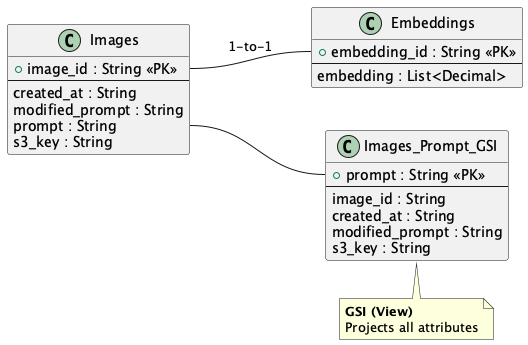
\includegraphics[width=0.6\textwidth]{uml/schemas.png} % Smaller image
    \caption{DynamoDB Schema and Relationships}
    \label{fig:schema}
\end{figure}

\section{API Design}

\begin{table}[h!]
\centering
\begin{tabular}{|l|l|l|l|}
\hline
\textbf{Endpoint} & \textbf{Method} & \textbf{Parameters} & \textbf{Description} \\ \hline
\texttt{/images} & GET & \texttt{prompt} (query, optional) & Generates a new image. \\
\texttt{/images/\{image\_id\}} & GET & \texttt{image\_id} (path) & Retrieves image and metadata. \\
\texttt{/images} & POST & \texttt{image\_data} (body, base64) & Uploads an image. \\
\texttt{/embeddings/\{embedding\_id\}} & GET & \texttt{embedding\_id} (path) & Retrieves/generates embedding. \\
\texttt{/similarity} & GET & \texttt{image\_id, prompt} (query) & Finds similar images. \\ \hline
\end{tabular}
\caption{API Endpoint Summary}
\label{tab:api_summary}
\end{table}

\noindent Detailed endpoint descriptions and sequence diagrams are provided below.

\subsection{GET /images}
Generates a new image from a text prompt using AWS Bedrock. Saves the image to S3 and writes metadata to DynamoDB. Appends random camera angle and style modifiers to the prompt.

\begin{itemize}[noitemsep,topsep=0pt,parsep=0pt,partopsep=0pt]
    \item \textbf{Success (200 OK):}
    \begin{lstlisting}
{
  "base_prompt": "...",
  "modified_prompt": "...",
  "image_id": "..."
}
    \end{lstlisting}
\end{itemize}

\begin{figure}[h!]
  \centering
  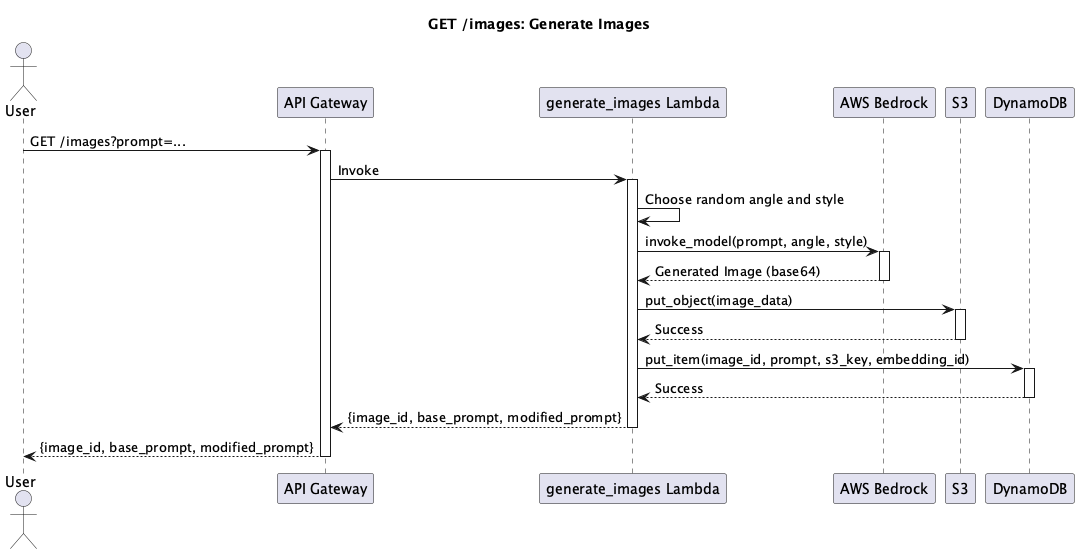
\includegraphics[width=0.7\textwidth]{uml/generate_images.png} % Smaller
  \caption{GET /images Sequence Diagram}
\end{figure}

\subsection{GET /images/\{image\_id\}}
Retrieves an image by ID. Returns metadata from DynamoDB and a presigned URL to S3.

\begin{itemize}[noitemsep,topsep=0pt,parsep=0pt,partopsep=0pt]
    \item \textbf{Success (200 OK):}
 \begin{lstlisting}
{
  "image_id": "...",
  "prompt": "...",
  "s3_key": "...",
  "url": "{presigned url to S3}"
}
\end{lstlisting}
\end{itemize}

\begin{figure}[h!]
    \centering
    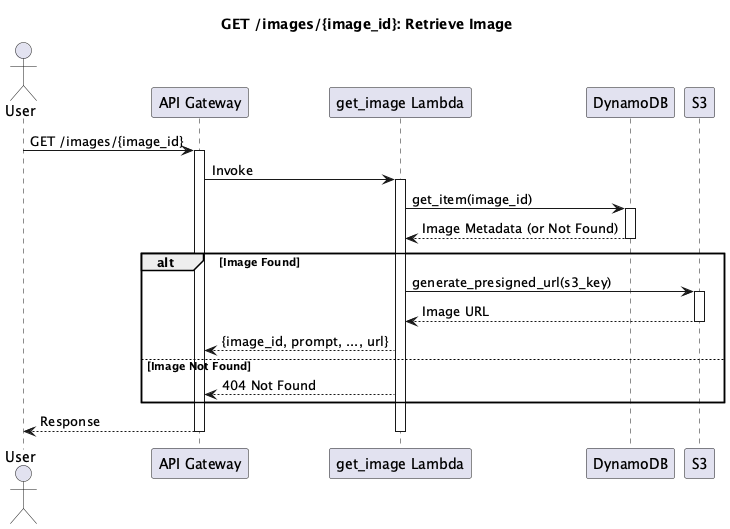
\includegraphics[width=0.7\textwidth]{uml/get_image.png} % Smaller
    \caption{GET /images/\{image\_id\} Sequence Diagram}
\end{figure}

\subsection{POST /images}
Uploads an image. Puts it to S3 and adds its metadata to DynamoDB.

\begin{itemize}[noitemsep,topsep=0pt,parsep=0pt,partopsep=0pt]
    \item \textbf{Success (200 OK):}
     \begin{lstlisting}
{
  "image_id": "...",
}
\end{lstlisting}
\end{itemize}

\begin{figure}[h!]
    \centering
    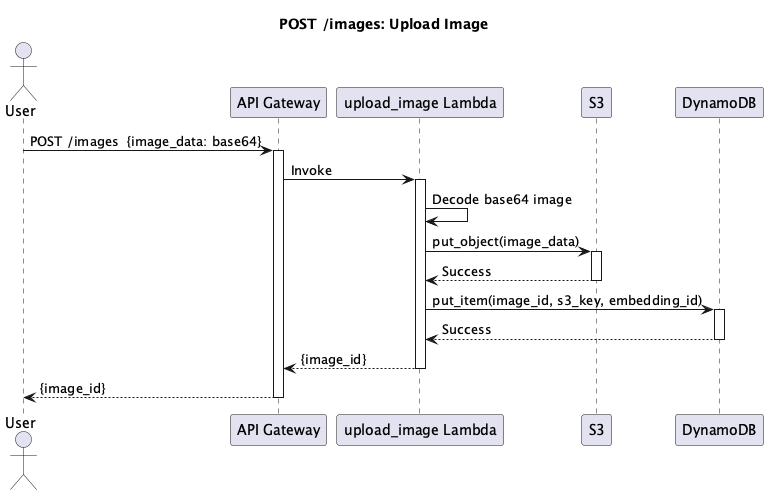
\includegraphics[width=0.7\textwidth]{uml/upload_image.png}% Smaller
    \caption{POST /images Sequence Diagram}
\end{figure}

\subsection{GET /embeddings/\{embedding\_id\}}
Retrieves an image embedding from DynamoDB. If it does not exist, fetches image from S3, generates embedding using CLIP model hosted on SageMaker, and writes the embedding to DynamoDB.

\begin{itemize}[noitemsep,topsep=0pt,parsep=0pt,partopsep=0pt]
    \item \textbf{Success (200 OK):}
         \begin{lstlisting}
{
  "embedding_id": "...",
  "embedding": [
    ...
  ]
}
\end{lstlisting}
\end{itemize}

\begin{figure}[h!]
    \centering
    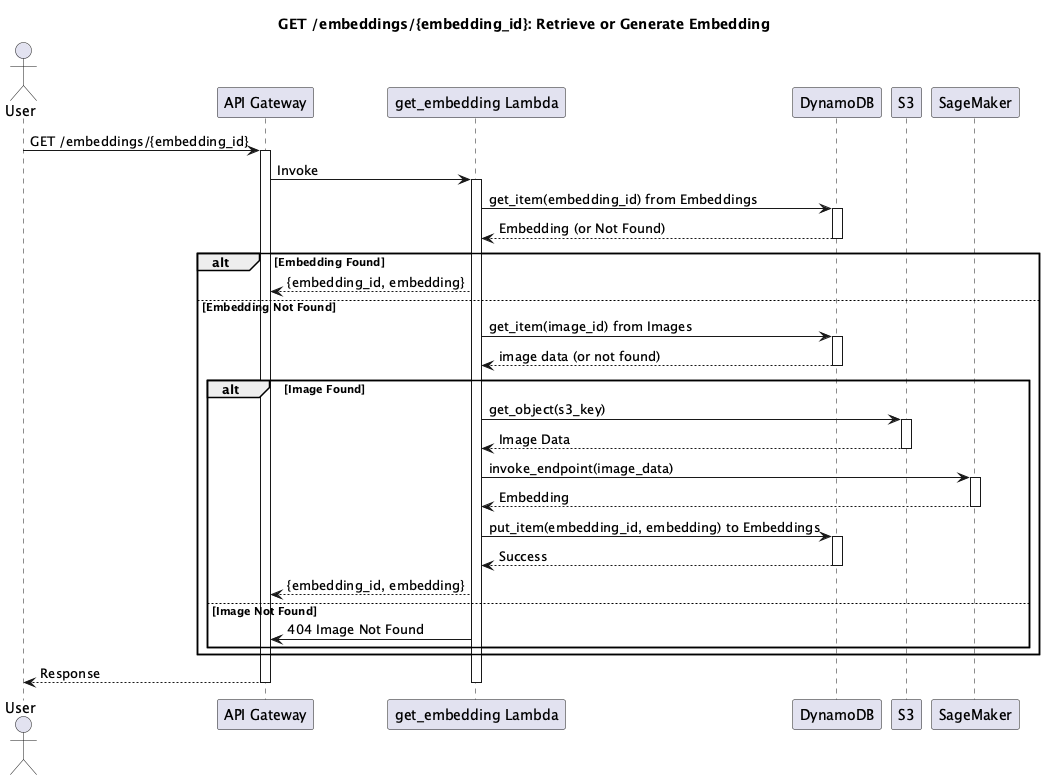
\includegraphics[width=0.7\textwidth]{uml/get_embedding.png}% Smaller
    \caption{GET /embedding/\{embedding\_id\} Sequence Diagram}
\end{figure}

\subsection{GET /similarity}
Finds similar images to a given image. Filters images compared to only images generated with a certain prompt, so as to compare between style and camera angle within one class of objects. Only searches through images that have embeddings already generated. Returns top 10 most similar matches, as determined by maximum cosine similarity.

\begin{itemize}[noitemsep,topsep=0pt,parsep=0pt,partopsep=0pt]

    \item \textbf{Success (200 OK):}
    \begin{samepage}
    \begin{lstlisting}
    {
      "results": [
            {
                "image_id": "...",
                "similarity": ...
            },
            ...
        ]
    }
    \end{lstlisting}
    \end{samepage}
\end{itemize}

\begin{figure}[h!]
    \centering
    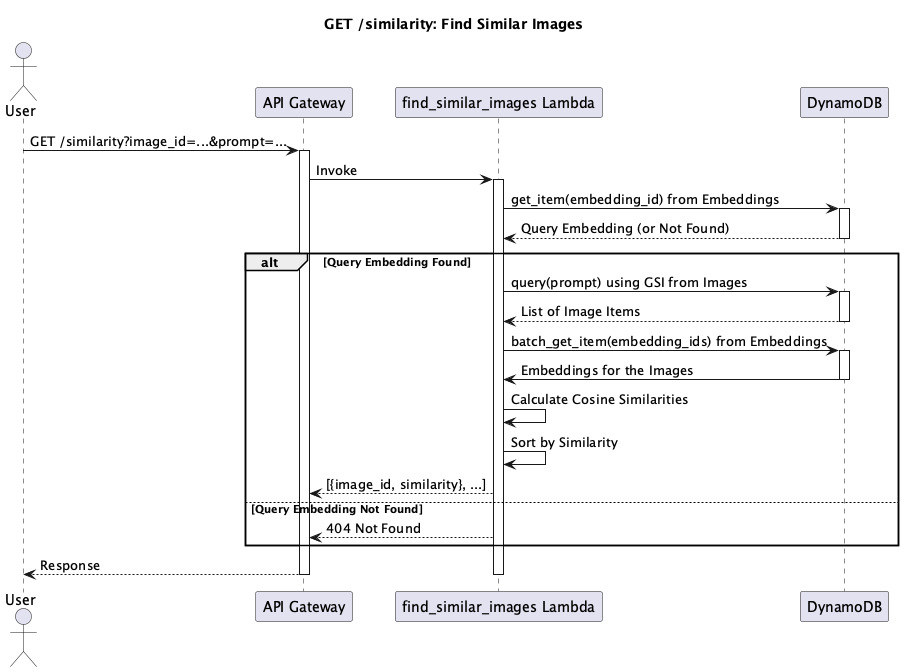
\includegraphics[width=0.7\textwidth]{uml/find_similar_images.png} % Smaller
    \caption{GET /similarity Sequence Diagram}
\end{figure}

\section{Database Schema}

The service uses two DynamoDB tables: `Images' and `Embeddings'. A Global Secondary Index `Images\_Prompt\_GSI`, allows filtering by prompt. See Fig. \ref{fig:schema}, Table \ref{tab:images_schema}, and Table \ref{tab:embeddings_schema}.

\begin{centering}
\begin{tabular}{|l|l|l|}
\hline
\textbf{Attribute} & \textbf{Type} & \textbf{Description} \\ \hline
\texttt{image\_id} & String & Unique image ID (Primary Key) \\
\texttt{created\_at} & String & Timestamp \\
\texttt{modified\_prompt} & String & Full prompt \\
\texttt{prompt} & String & Base prompt \\
\texttt{s3\_key} & String & S3 path \\ \hline
\end{tabular}
\captionof{table}{Images Table Schema}
\label{tab:images_schema}

\vspace{1em}

\begin{tabular}{|l|l|l|}
\hline
\textbf{Attribute} & \textbf{Type} & \textbf{Description} \\ \hline
\texttt{embedding\_id} & String & Embedding ID (Primary Key) \\
\texttt{embedding} & List\textlangle Decimal\textrangle & Embedding vector \\ \hline
\end{tabular}
\captionof{table}{Embeddings Table Schema}
\label{tab:embeddings_schema}
\end{centering}

% \begin{figure}[h!]
%     \centering
%     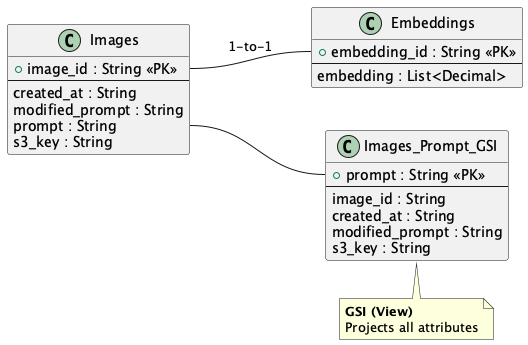
\includegraphics[width=0.6\textwidth]{uml/schemas.png} % Smaller image
%     \caption{DynamoDB Schema and Relationships}
%     \label{fig:schema}
% \end{figure}


\end{document}
